\documentclass[11pt]{article}

\usepackage[margin=1in]{geometry}
\usepackage{graphicx}
\usepackage{booktabs}
\usepackage{amsmath,amssymb}
\usepackage{microtype}
\usepackage[colorlinks,citecolor=blue,urlcolor=blue,linkcolor=blue]{hyperref}
\usepackage{xcolor}
\usepackage{enumitem}
\usepackage{caption}

\setlength{\parskip}{0.5em}
\setlength{\parindent}{0em}

\newcommand{\real}{\mathbb{R}}
\newcommand{\expect}{\mathbb{E}}
\newcommand{\kl}{D_{\mathrm{KL}}}
\newcommand{\occ}{\Phi}
\newcommand{\zlat}{z}
\newcommand{\tred}{\tau^{\mathrm{red}}}

\title{Three Preconditions for Latent Opponent Modeling in\\
Adversarial Co-Training: An Empirical Study in a\\
Resource-Augmented Predator--Prey Game}
\author{Rajdeep Singh \\ REL Lab, University of Southern California}
\date{May 2026}

\begin{document}
\maketitle

\begin{abstract}
We are building toward an adversarial co-training method in which one team
(\emph{blue}) plans against a learned, uncertainty-aware model of its opponent
(\emph{red}): a variational encoder maps a red trajectory to a latent strategy
variable $\zlat$, a latent-conditioned policy reconstructs red's behavior, and a
model-based planner samples that policy at each search node. The method rests on
three empirical preconditions that are usually \emph{assumed}: (P1) the opponent
exhibits genuinely distinct strategies; (P2) those strategies are recoverable by
an unsupervised encoder into a latent that separates them; and (P3) a strong
co-trained best response is actually brittle to an out-of-distribution opponent,
so that opponent-aware planning has something to fix. We test all three in a
resource-augmented predator--prey game (\texttt{SimpleTagResourcesMPE}, JaxMARL).
A prior experiment found that a \emph{dominated} prey expresses its
resource-collection strategy only as a weak aggregate perturbation, blocking all
three. Restoring a balanced regime---specialist prey co-trained on a single
resource layout, with predator speed reduced so the prey can execute a
route---makes all three preconditions hold: the circle- and corners-specialist
prey trace a diamond and a square respectively, separable from occupancy at
$0.98$ (chance $0.50$); an unsupervised VAE on the trajectory occupancy
histogram recovers the strategy with adjusted Rand index $0.87$ and a latent
linear-probe accuracy of $0.99$ given $\geq 100$ steps of observation; and MAPPO
predators co-trained against one prey suffer a $43\%$ drop in capture rate when
faced with the unseen prey. Building on these, we realize the proposal's Part~1:
a single behavior-cloned policy $\pi_\psi(a \mid s, \zlat)$ that reproduces either
specialist by swapping its latent, whose route is controllable by $\zlat$ at
$0.85$ even with the environment held fixed. We give the formal setup, the
encoder and cloning objectives, and the metric definitions, and discuss the
regime-dependence of each result.
\end{abstract}


%% ==================================================================
\section{Introduction}

In adversarial multi-agent reinforcement learning (MARL), each team faces a
non-stationary environment because the opposing team is itself learning. A
recurring failure mode is \emph{overfitting to the opponent}: a team learns a
best response to its current adversary and loses robustness to strategies it has
not recently seen. The method this paper supports addresses that failure by
giving the planning team an explicit, uncertainty-aware model of its opponent.
Concretely (Parts~1--2 of the proposal):

\begin{description}[style=nextline,font=\normalfont\bfseries,leftmargin=1.2em]
\item[Part 1 (encoder).] A variational encoder
$q_\phi(\zlat \mid \tred)$ maps a red (opponent) trajectory $\tred$ to a latent
strategy variable $\zlat$, trained by maximizing an evidence lower bound (ELBO).
A latent-conditioned policy $\pi^{\mathrm{red}}_\psi(a \mid s, \zlat)$ then
reconstructs red's behavior, by behavior cloning or contrastive preference
learning.
\item[Part 2 (planner).] A model-based (MuZero-style) planner expands a search
tree in which blue actions branch and red actions are \emph{sampled} from
$\pi^{\mathrm{red}}_\psi(\cdot \mid s, \zlat)$, with a latent-conditioned value
function $v^{\mathrm{blue}}(s, \zlat)$ scoring nodes.
\end{description}

This machinery is only worth building if three things are true of the domain.
The opponent must \emph{have} distinct strategies to model (P1); those strategies
must be \emph{encodable} into $\zlat$ by an unsupervised objective (P2); and the
co-trained policy we intend to improve must in fact be \emph{brittle} to
out-of-distribution opponents (P3), or there is nothing for opponent-aware
planning to fix. This paper isolates and tests P1--P3 directly, before investing
in the encoder--planner stack.

\paragraph{Prior negative result.}
An earlier experiment built a resource-augmented predator--prey task expressly to
make strategy separable, then found the separation absent: a single prey trained
on a \emph{mixed} circle/corners placement produced trajectories whose layout was
not recoverable even by a supervised probe (accuracy $\approx$ chance), and an
unsupervised trajectory VAE reached adjusted Rand index ARI $\approx 0.008$
against the placement label---essentially the same null as the earlier
reward-shaping study. We trace this to opponent \emph{domination}: three
coordinated predators force the prey into near-pure evasion across the whole
arena, so the resource layout perturbs its occupancy only weakly and never on a
single trajectory. The contribution here is to show that, in a balanced regime
where the prey expresses its strategy, all three preconditions hold, with the
formal setup and metrics needed to state them precisely.


%% ==================================================================
\section{Problem setup}

\subsection{Markov game}

We model the task as a partially observed Markov game
$\langle \mathcal{N}, \mathcal{S}, \{\mathcal{A}_i\}, \{\mathcal{O}_i\}, P, \{R_i\}, \gamma \rangle$
with agents $\mathcal{N} = P \cup \{q\}$ split into a predator team
$P = \{1,2,3\}$ and a single prey $q$. At step $t$, agent $i$ receives an
observation $o^t_i \in \mathcal{O}_i$, selects a discrete action
$a^t_i \in \mathcal{A}_i = \{\text{stay},\,\leftarrow,\,\rightarrow,\,\downarrow,\,\uparrow\}$,
and the joint action drives the MPE point-mass dynamics
$s^{t+1} \sim P(\cdot \mid s^t, a^t)$. Episodes last $H = 25$ steps. Predators
share weights within the team; the two teams are trained as separate
actor--critic (MAPPO) or $Q$-learning (IQL) pairs, so the game is adversarial,
not cooperative.

\subsection{Rewards}

Let $\mathbf{1}[\cdot]$ be the indicator and write $c^t_{i} = \mathbf{1}\!\left[
\lVert x^t_i - x^t_q \rVert < \rho_i + \rho_q \right]$ for the event that
predator $i$ is in contact with the prey at step $t$, where $x$ are positions and
$\rho$ are body radii. The predator team receives a \emph{shared} reward
proportional to the number of predators in contact,
\begin{equation}
  r^{\mathrm{pred},t} \;=\; \lambda_{\mathrm{tag}} \sum_{i \in P} c^t_i,
  \qquad \lambda_{\mathrm{tag}} = 10,
  \label{eq:rpred}
\end{equation}
and every predator receives this same value. The prey receives the negative tag
reward, a boundary penalty $b(x^t_q) \geq 0$ discouraging it from leaving the
arena, and a collection bonus:
\begin{equation}
  r^{\mathrm{prey},t} \;=\; -\,\lambda_{\mathrm{tag}} \sum_{i \in P} c^t_i
  \;-\; b(x^t_q)
  \;+\; \lambda_{\mathrm{col}} \sum_{j=1}^{4} \Delta^t_j,
  \label{eq:rprey}
\end{equation}
where $\Delta^t_j \in \{0,1\}$ marks resource $j$ being collected for the first
time at step $t$. A resource is collected when the prey approaches within
$r_{\mathrm{col}} = 0.15$; only the prey observes resource positions and only the
prey can collect. We define \emph{captures per episode} as the episode tag count
recovered from the shared predator return,
\begin{equation}
  \mathrm{cap} \;=\; \frac{1}{\lambda_{\mathrm{tag}}}
  \sum_{t=1}^{H} r^{\mathrm{pred},t}.
  \label{eq:captures}
\end{equation}

\subsection{Resource layouts}

Four resources are placed at reset according to a layout $\ell$:
\begin{equation}
  \text{circle:}\quad g_j = 0.6\,(\cos\theta_j, \sin\theta_j),\;
  \theta_j = \tfrac{\pi}{2} j;
  \qquad
  \text{corners:}\quad g_j \in \{\pm 0.8\}^2 .
\end{equation}
The two layouts induce different optimal collection routes---a loop around the
ring versus a tour of the four corners---which is the strategy signal P1--P3 are
about. Two fixed obstacles sit at $(\pm 0.5, \pm 0.5)$.

\subsection{The encoder we are building toward}

Part~1 learns $q_\phi(\zlat \mid \tred)$ and a decoder $p_\theta(\tred \mid
\zlat)$ by maximizing the ELBO
\begin{equation}
  \mathcal{L}(\phi,\theta)
  = \underbrace{\expect_{q_\phi(\zlat \mid \tred)}
      \big[\log p_\theta(\tred \mid \zlat)\big]}_{\text{reconstruction}}
  \;-\; \underbrace{\kl\!\big(q_\phi(\zlat \mid \tred)\,\Vert\,p(\zlat)\big)}_{\text{regularizer}},
  \qquad p(\zlat) = \mathcal{N}(0, I).
  \label{eq:elbo}
\end{equation}
P2 below is exactly the question of whether the latent learned by
Eq.~\eqref{eq:elbo} separates red's strategies. A key empirical choice, motivated
by the prior negative result, is the encoder \emph{input}. A raw position
sequence is dominated by evasion and start-position noise; the layout signal
lives in \emph{where} the prey spends time. We therefore featurize a trajectory
$\tau = (x^1,\dots,x^L)$ by its normalized 2D occupancy histogram over a
$B \times B$ grid on $[-1.6, 1.6]^2$,
\begin{equation}
  \occ_B(\tau)_{kl} = \frac{1}{L}\sum_{t=1}^{L}
    \mathbf{1}\!\left[x^t \in \mathrm{bin}_{kl}\right]
  \;\in\; \Delta^{B^2-1},
  \qquad B = 12,
  \label{eq:occ}
\end{equation}
and use $\occ_B(\tau)$ as the input to the encoder of Eq.~\eqref{eq:elbo}.


%% ==================================================================
\section{The three preconditions as measurable hypotheses}

\paragraph{Metrics.}
For a feature map $\varphi$ and binary placement labels $y \in \{0,1\}$ (circle
vs corners, recovered from resource geometry and never shown to any encoder), the
\emph{linear-probe accuracy} $\mathrm{Acc}(\varphi)$ is the 5-fold
cross-validated accuracy of $\ell_2$-regularized logistic regression predicting
$y$ from $\varphi$. For an unsupervised clustering $\hat y$ (here a two-component
Gaussian mixture fit to the latent $\zlat$), the \emph{adjusted Rand index}
$\mathrm{ARI}(\hat y, y) \in [-1,1]$ measures agreement with the true labels
corrected for chance ($0$ at chance, $1$ for a perfect match). We state each
precondition as a hypothesis with its estimator:
\begin{description}[style=nextline,font=\normalfont\bfseries,leftmargin=1.2em]
\item[P1 (distinct strategies).] $\mathrm{Acc}\big(\occ_B(\tau)\big) \gg 0.5$:
the placement is linearly decodable from a trajectory's occupancy, i.e.\ the two
specialists occupy the arena differently.
\item[P2 (encodable).] For $\zlat \sim q_\phi(\cdot \mid \occ_B(\tau))$ trained
\emph{unsupervised} by Eq.~\eqref{eq:elbo}, both $\mathrm{Acc}(\zlat) \gg 0.5$
(the latent retains strategy) and $\mathrm{ARI} \gg 0$ (an unsupervised reading
of the latent recovers it).
\item[P3 (brittleness).] Let $M_{\ell\ell'} = \expect[\mathrm{cap}]$ when a
predator co-trained on layout $\ell$ faces a prey co-trained on layout $\ell'$,
each in its native layout. Then the in-distribution (diagonal) mean exceeds the
out-of-distribution (off-diagonal) mean:
$\bar M_{\mathrm{in}} = \tfrac12(M_{cc} + M_{kk})
> \bar M_{\mathrm{ood}} = \tfrac12(M_{ck} + M_{kc})$.
We report the relative brittleness
$\beta = 1 - \bar M_{\mathrm{ood}} / \bar M_{\mathrm{in}}$.
\end{description}

\subsection{Experimental regime}

To make red express strategy we (i) train \emph{specialists}: a separate
predator+prey co-training run on each fixed layout (circle-only, corners-only),
three seeds each; and (ii) balance the game so the prey is not dominated, by
reducing predator top speed $1.0 \to 0.6$ and acceleration $3.0 \to 1.5$ (prey
unchanged at $1.3 / 4.0$) and raising the collection bonus
$\lambda_{\mathrm{col}}: 5 \to 10$. All other settings match the base task.
IQL/OA-IQL use a 128-unit MLP, replay buffer $5000$, batch $32$,
$\epsilon: 1.0 \to 0.05$, $\gamma = 0.9$, learning rate $0.005$. MAPPO uses a
per-team actor with a centralized critic over the concatenated team observation,
$32$ environments $\times\, 128$ steps, $4$ PPO epochs, $\gamma = 0.99$,
$\lambda_{\mathrm{GAE}} = 0.95$. Evaluation uses $200$ greedy episodes per cell
for P3 and $300$ trajectories per specialist for P1/P2.


%% ==================================================================
\section{Results}

\subsection{P1 --- different layouts produce different strategies}

The two specialists trace visibly different routes
(Figure~\ref{fig:p1}): the circle-prey loops a diamond between the four ring
resources, the corners-prey patrols a square around the perimeter. Pooling each
trajectory into its occupancy histogram (Eq.~\ref{eq:occ}), placement is linearly
decodable at $\mathrm{Acc} = 0.98$ for the IQL prey and $0.96$ for MAPPO, against
a chance rate of $0.50$ (Table~\ref{tab:p1}). P1 holds.

\begin{figure}[h]
  \centering
  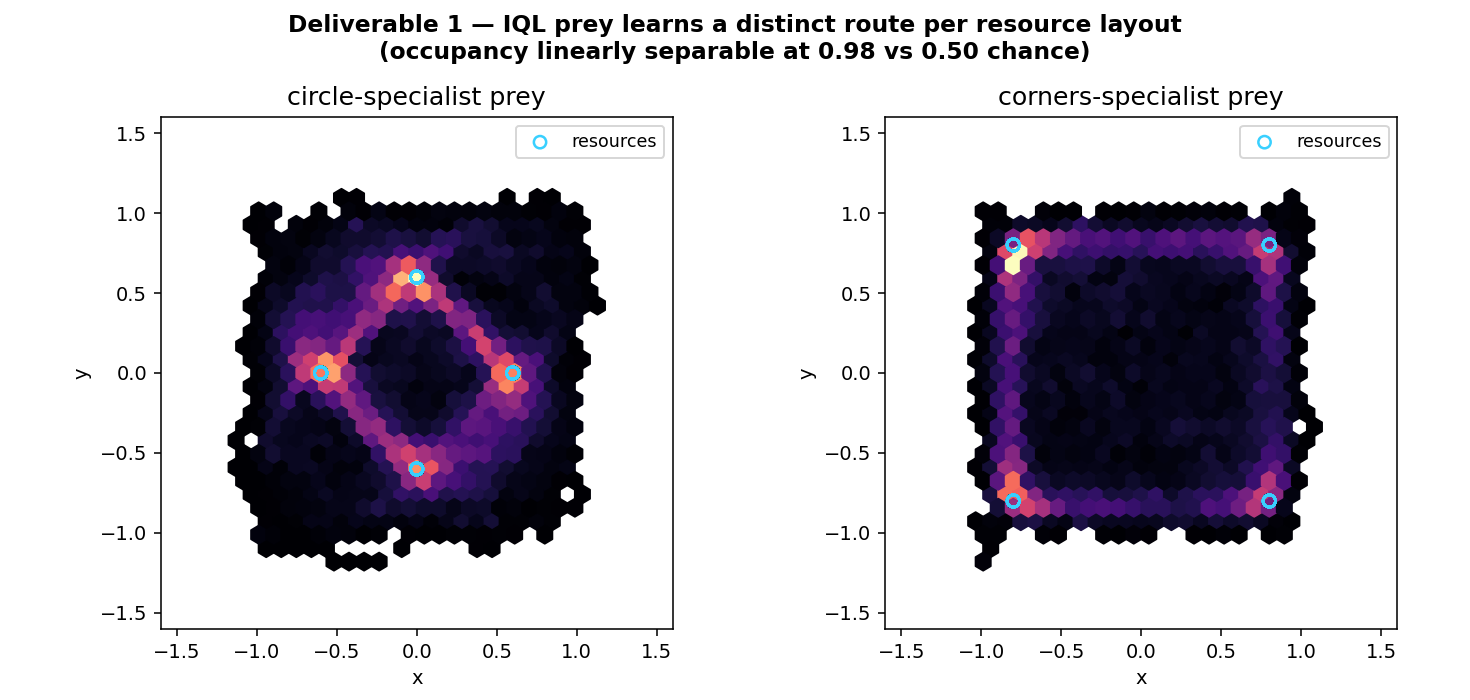
\includegraphics[width=\textwidth]{../plots/exp5_specialist_iql_wp.png}
  \caption{\textbf{P1.} Prey occupancy density (pooled over $300$ episodes per
  specialist; cyan rings mark resource positions). The circle-specialist's route
  is a diamond between ring resources; the corners-specialist's is a perimeter
  square. Occupancy is linearly separable at $0.98$.}
  \label{fig:p1}
\end{figure}

\begin{table}[h]
  \centering
  \caption{\textbf{P1.} Linear-probe placement accuracy from a single
  trajectory's occupancy histogram (chance $= 0.50$).}\label{tab:p1}
  \begin{tabular}{@{}lcc@{}}
    \toprule
    Prey policy & Occupancy-probe accuracy & Chance \\
    \midrule
    IQL specialist   & $\mathbf{0.98}$ & 0.50 \\
    MAPPO specialist & $0.96$          & 0.50 \\
    \midrule
    \emph{(prior) mixed-placement prey} & $\approx 0.50$ & 0.50 \\
    \bottomrule
  \end{tabular}
\end{table}

\subsection{P2 --- an unsupervised latent that encodes the strategy}

We train the VAE of Eq.~\eqref{eq:elbo} on occupancy histograms
(Eq.~\ref{eq:occ}) with no labels, and sweep the observation length $L$ used to
build each histogram. Recovery rises monotonically with $L$
(Table~\ref{tab:p2}, Figure~\ref{fig:p2}): by $L = 100$ steps the IQL prey's
latent gives a supervised probe of $0.99$ and an \emph{unsupervised} ARI of
$0.87$, i.e.\ a two-component mixture on the latent recovers the placement almost
perfectly. P2 holds for the IQL prey. For the MAPPO prey---more dominated even in
the balanced regime---the latent retains strategy supervised (probe $0.83$) but
does not separate unsupervised (ARI $\approx 0$); cleaner strategy expression
yields a cleaner latent.

\begin{table}[h]
  \centering
  \caption{\textbf{P2.} Placement recovery from the unsupervised VAE latent as a
  function of observation length $L$ (IQL specialists). Occupancy-probe is the
  supervised upper bound on the histogram; latent-probe and ARI read the
  unsupervised latent.}\label{tab:p2}
  \begin{tabular}{@{}lcccc@{}}
    \toprule
    & $L=25$ & $L=50$ & $L=75$ & $L=100$ \\
    \midrule
    Occupancy-probe (supervised) & 0.93 & 0.96 & 0.98 & $\mathbf{1.00}$ \\
    Latent-probe (supervised)    & 0.59 & 0.89 & 0.94 & $\mathbf{0.99}$ \\
    Latent ARI (unsupervised)    & 0.07 & 0.44 & 0.79 & $\mathbf{0.87}$ \\
    \bottomrule
  \end{tabular}
\end{table}

\begin{figure}[h]
  \centering
  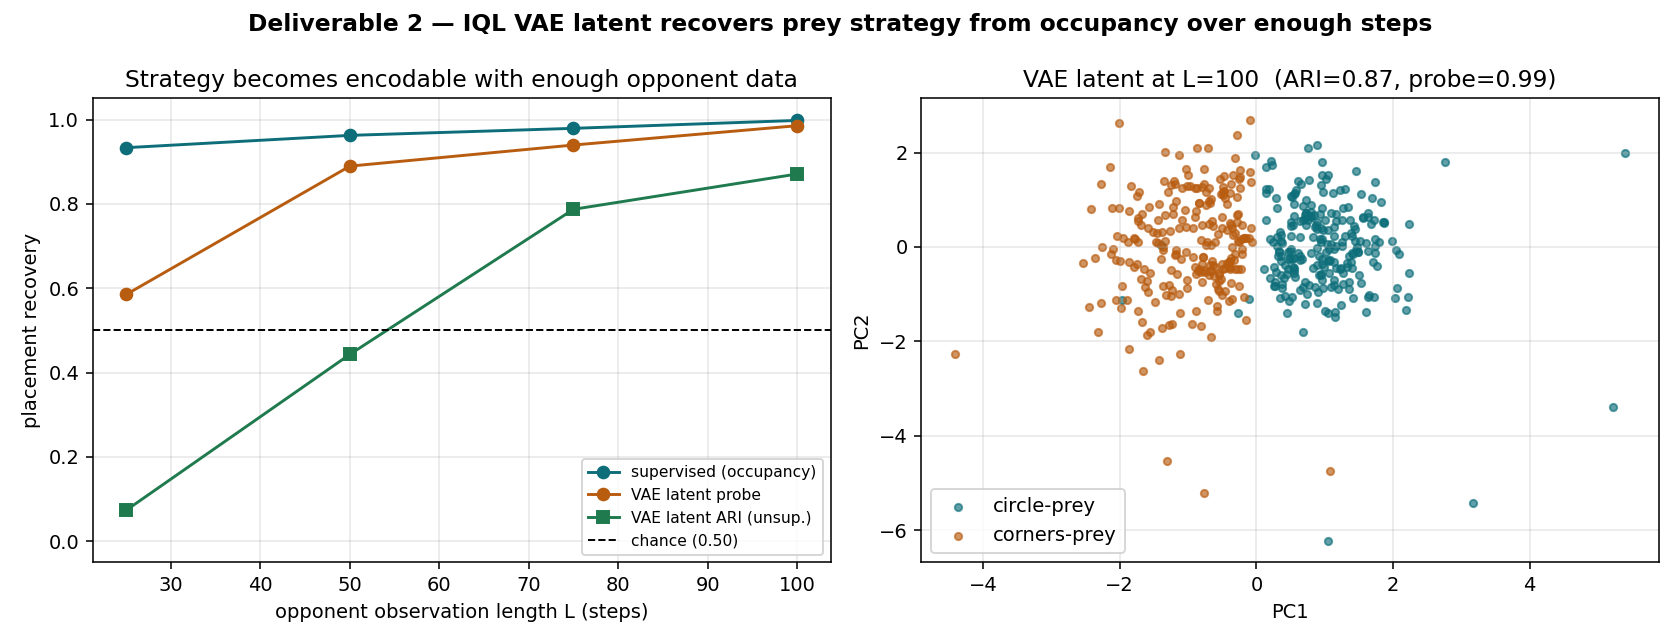
\includegraphics[width=\textwidth]{../plots/exp5b_encoder_length_iql_wp.png}
  \caption{\textbf{P2.} Left: placement recovery vs.\ observation length;
  supervised occupancy-probe, supervised latent-probe, and unsupervised ARI all
  rise with $L$. Right: the unsupervised VAE latent at $L = 100$ forms two
  clusters aligned with circle vs.\ corners (ARI $0.87$), trained without
  labels.}
  \label{fig:p2}
\end{figure}

Past $L \approx 150$ the occupancy histogram saturates (the prey covers the whole
arena) and the unsupervised ARI degrades even though the supervised latent-probe
stays at $0.99$; there is an intermediate observation window that is optimal for
unsupervised strategy discovery. This is consistent with the planner needing a
\emph{sufficient but bounded} window of opponent observation to infer $\zlat$.

\subsection{P3 --- co-trained predators are brittle to an unseen opponent}

Table~\ref{tab:p3} is the $2\times2$ cross-play matrix $M$ of captures per
episode (Eq.~\ref{eq:captures}) for the MAPPO specialists; Figure~\ref{fig:p3}
visualizes it. Reading column-wise holds the prey and its environment fixed and
swaps only the predator, isolating the predator's contribution: the
circle-prey is caught $1.90$ times per episode by its co-trained predator but
only $1.11$ by the unfamiliar one; the corners-prey, $1.29$ vs.\ $0.72$. The
in-distribution mean is $\bar M_{\mathrm{in}} = 1.59$ and the
out-of-distribution mean is $\bar M_{\mathrm{ood}} = 0.91$, a relative
brittleness of $\beta = 0.43$. P3 holds for MAPPO. The IQL predators are too
generic to specialize ($\bar M_{\mathrm{in}} = 0.26$ vs.\
$\bar M_{\mathrm{ood}} = 0.24$, $\beta = 0.07$), so brittleness is a property of
the strong centralized-critic predator---precisely the policy class the
opponent-aware planner is meant to improve.

\begin{table}[h]
  \centering
  \caption{\textbf{P3.} Captures per episode (mean $\pm$ std over 3 seeds,
  $200$ episodes each), MAPPO specialists. Rows: predator's training layout;
  columns: prey's training layout (each prey in its native environment).
  Diagonal $=$ in-distribution, off-diagonal $=$ out-of-distribution
  prey.}\label{tab:p3}
  \begin{tabular}{@{}lcc@{}}
    \toprule
    & prey: circle & prey: corners \\
    \midrule
    pred: circle  & $\mathbf{1.90 \pm 0.17}$ & $0.72 \pm 0.08$ \\
    pred: corners & $1.11 \pm 0.28$          & $\mathbf{1.29 \pm 0.37}$ \\
    \bottomrule
  \end{tabular}
\end{table}

\begin{figure}[h]
  \centering
  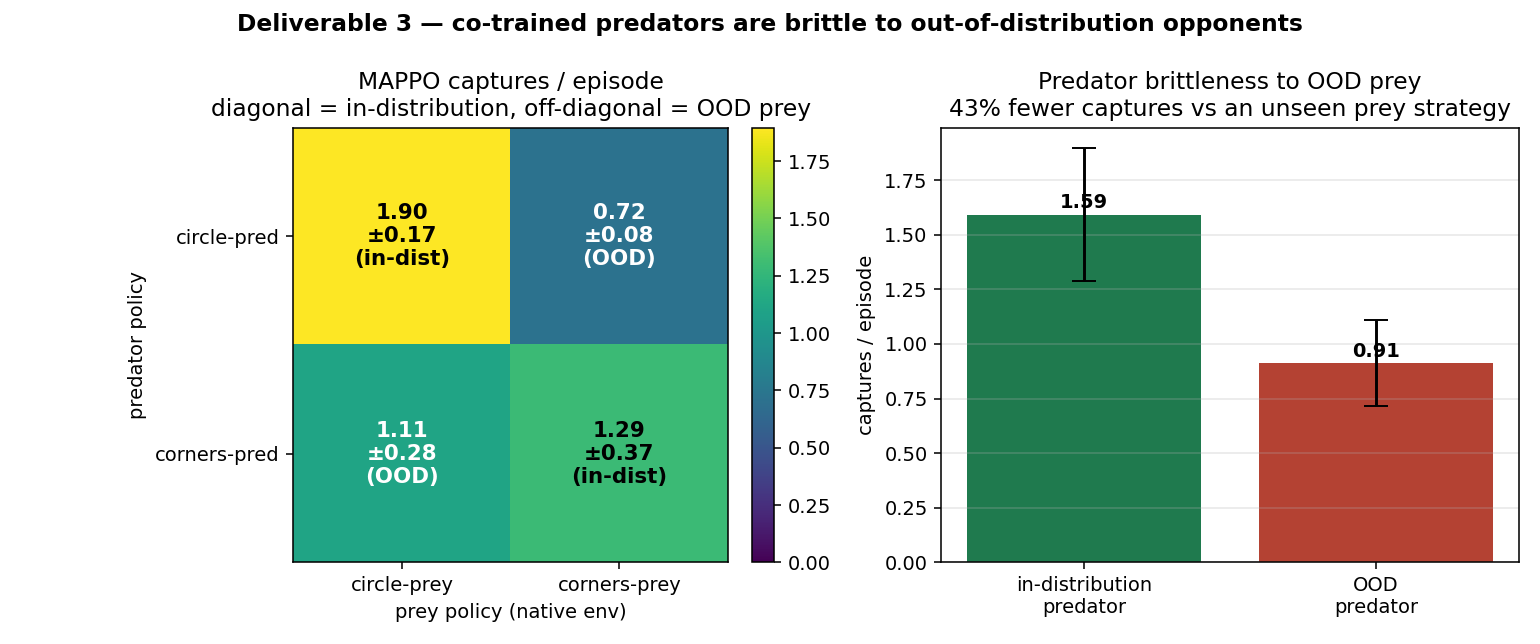
\includegraphics[width=\textwidth]{../plots/brittleness_mappo_wp.png}
  \caption{\textbf{P3.} Left: the cross-play matrix of captures/episode; the
  in-distribution diagonal is brighter than the OOD off-diagonal. Right: averaged
  over pairings, the co-trained predator catches $43\%$ more than the unfamiliar
  one ($1.59 \to 0.91$).}
  \label{fig:p3}
\end{figure}


%% ==================================================================
\section{Discussion}

\paragraph{Regime dependence is the point, not a caveat.}
None of P1--P3 hold for the dominated prey of the prior experiment; all hold once
the prey is allowed to express strategy. This is expected and, in fact, defines
where opponent modeling is useful: an opponent that cannot vary its behavior has
no strategy to infer, and a planner gains nothing by modeling it. The balanced,
specialist regime is the operating point at which the proposal's machinery is
both necessary and applicable.

\paragraph{A division of labor between algorithms.}
The cleanest \emph{encodable} strategy comes from the value-based prey (P1, P2),
whose weaker predators let it execute full routes; the cleanest
\emph{brittleness} comes from the MAPPO predator (P3), whose centralized critic
learns a layout-specific interception that does not transfer. This is coherent:
P1/P2 require red to express strategy, while P3 requires blue to be strong enough
to overfit to it. A latent-conditioned planner is the bridge---it gives a
decentralized executor access to the opponent structure that a centralized critic
otherwise exploits only during training.

\paragraph{Representation and observation length.}
Two design choices were decisive for P2 and both transfer to the planned encoder.
First, occupancy (Eq.~\ref{eq:occ}) rather than the raw position sequence: the
strategy is in \emph{where} the opponent goes, and a reconstruction objective on
ordered positions spends its capacity on evasion noise. Second, a sufficient
observation window: separability is monotone in $L$ up to saturation, so the
planner's belief over $\zlat$ should sharpen as red is observed and then be
capped before the occupancy washes out.


%% ==================================================================
\section{Part 1 realized: a latent-conditioned opponent model}

With P1--P3 established we build the proposal's Part~1 directly: a single prey
policy $\pi^{\mathrm{red}}_\psi(a \mid s, \zlat)$ that reproduces either
specialist by conditioning on the latent. Let $z_\phi(\tau) = \mu_\phi(\occ_B(\tau))$
be the encoder's posterior mean (Eq.~\ref{eq:elbo}, the same $Z = 3$ occupancy
VAE as P2). We log $(s_t, a_t)$ pairs from the circle- and corners-specialist
rollouts, tag each pair with its trajectory's code, and minimize the
behavior-cloning loss
\begin{equation}
  \mathcal{L}_{\mathrm{BC}}(\psi)
  = -\,\expect_{\tau \sim \mathcal{D}}\;
      \expect_{(s_t,a_t)\in\tau}
      \Big[\log \pi^{\mathrm{red}}_\psi\!\big(a_t \mid s_t,\, z_\phi(\tau)\big)\Big].
  \label{eq:bc}
\end{equation}
We then form class-mean codes $\bar z_\ell = \expect_{\tau \in \ell}[z_\phi(\tau)]$
and probe \emph{latent controllability}: roll $\pi^{\mathrm{red}}_\psi$ out with
$\zlat$ \emph{clamped} to $\bar z_{\mathrm{circle}}$ vs.\ $\bar z_{\mathrm{corners}}$
and measure whether the resulting routes differ. We report this both
across matched environments (each $\bar z_\ell$ in its native layout) and, more
stringently, in a \emph{fixed} environment with the same predators, where only
$\zlat$ changes; the latter isolates the latent's effect from the observation.

\begin{table}[h]
  \centering
  \caption{\textbf{Part 1.} Latent-conditioned BC (IQL prey). Action-match is
  held-out accuracy of $\arg\max_a \pi_\psi(a \mid s, z_\phi(\tau))$ against the
  specialist's action; route separation is the occupancy-probe accuracy
  separating the two clamped-$\zlat$ rollouts (chance $0.50$).}\label{tab:part1}
  \begin{tabular}{@{}lcc@{}}
    \toprule
    Quantity & Value & Baseline / chance \\
    \midrule
    BC action-match (held-out)               & $0.62$ & $0.24$ (majority action) \\
    Encoder separates specialists            & $0.96$ & $0.50$ \\
    Route sep., matched env ($\bar z_\ell$)  & $\mathbf{1.00}$ & $0.50$ \\
    Latent control, fixed env (swap $\zlat$) & $\mathbf{0.85}$ & $0.50$ \\
    \bottomrule
  \end{tabular}
\end{table}

\begin{figure}[h]
  \centering
  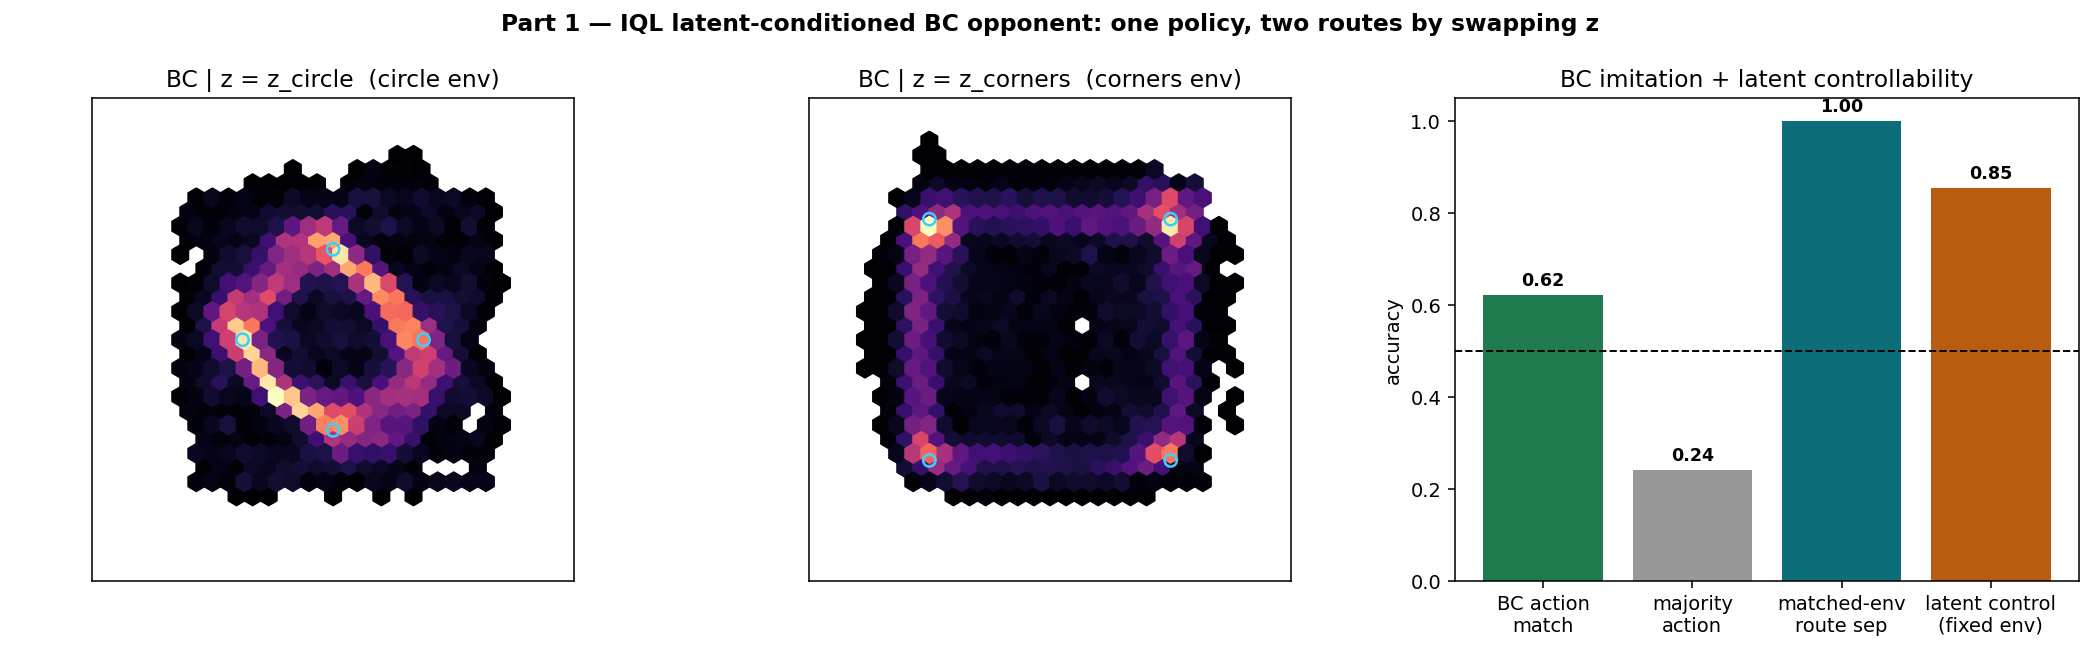
\includegraphics[width=\textwidth]{../plots/part1_latent_bc_iql.png}
  \caption{\textbf{Part 1.} One BC policy, two routes by swapping the latent.
  Left/middle: occupancy of $\pi^{\mathrm{red}}_\psi$ clamped to
  $\bar z_{\mathrm{circle}}$ (a diamond) and $\bar z_{\mathrm{corners}}$ (a
  square). Right: action-match exceeds the majority-action baseline, and the
  latent controls the route even with the environment held fixed ($0.85$).}
  \label{fig:part1}
\end{figure}

The policy clones each specialist's action at $0.62$ held-out accuracy (vs.\ a
$0.24$ majority-action floor; the residual is the specialist's own stochasticity
given $s$), and---decisively for the planner---swapping $\zlat$ alone steers the
prey's route at $0.85$ in a fixed environment (Table~\ref{tab:part1},
Figure~\ref{fig:part1}). This is the controllable opponent model Part~2 requires.


%% ==================================================================
\section{Outlook: Part 2}

\textbf{Part 2} embeds $\pi^{\mathrm{red}}_\psi(\cdot \mid s, \zlat)$ as the
red-action sampler in a MuZero-style search and conditions the blue value
function on $\zlat$ inferred from observed red play; the contrastive-preference
variant replaces Eq.~\eqref{eq:bc} with a Bradley--Terry objective whose negative
trajectories are generated by the planner itself. P3 gives the concrete target,
recovering on the OOD diagonal the captures a co-trained predator loses: the
headline numbers to beat are in Table~\ref{tab:p3}---an opponent-aware
circle-predator should catch the corners-prey closer to the in-distribution
$1.29$ than the unaware $0.72$.

\end{document}
